\documentclass[11pt,aspectratio=43]{beamer}
\usepackage[utf8]{inputenc}
\usepackage{amsmath, amsfonts, amssymb, amsthm}
\usepackage[T1]{fontenc}
\usepackage{lmodern}
\usepackage{xcolor}
\usepackage{setspace}
\usepackage{booktabs}
\usepackage{multirow}
\usepackage{graphicx}
\usepackage{tikz}
% \usetikzlibrary{decorations}
\usetikzlibrary{decorations.pathreplacing}
\usepackage{ulem}
\usepackage{hyperref}
\usepackage{booktabs}
\usepackage{babel}
\usepackage{makecell}
\usepackage[para,online,flushleft]{threeparttable}
\usepackage{pdfpages}
\usepackage{tcolorbox}
\usepackage{bm}
\usepackage{appendixnumberbeamer}
\usepackage{natbib}
\usepackage{caption}
\captionsetup[figure]{labelformat=empty}% redefines the caption setup of the figures environment in the beamer class.
\usetheme[compress]{Boadilla}
\usecolortheme{default}
\useoutertheme{miniframes}
\usefonttheme[onlymath]{serif}

\newcommand{\jump}[2]{\hyperlink{#1}{\beamerbutton{#2}}}
\newcommand{\orange}[1]{\textcolor{orange}{#1}}
\newcommand{\red}[1]{\textcolor{red}{#1}}

\setbeamertemplate{itemize item}{\raisebox{0.1em}{\scalebox{0.7}{$\blacksquare$}}}
\setbeamertemplate{itemize subitem}[circle]
\setbeamertemplate{itemize subsubitem}{--}
\setbeamercolor{itemize item}{fg=black}
\setbeamercolor{itemize subitem}{fg=black}
\setbeamercolor{itemize subsubitem}{fg=black}
\setbeamercolor{item projected}{bg=darkgray,fg=white}
\definecolor{blue}{rgb}{0.2, 0.2, 0.7}
\setbeamercolor{alerted text}{fg=blue}
\setbeamertemplate{enumerate items}[circle]


\setbeamertemplate{headline}{}

%==========================================
\let\olditemize=\itemize
\let\endolditemize=\enditemize
\renewenvironment{itemize}{\olditemize \itemsep1em}{\endolditemize}
\let\oldenumerate=\enumerate
\let\endoldenumerate=\endenumerate
\renewenvironment{enumerate}{\oldenumerate \itemsep1em}{ \endoldenumerate}

\DeclareMathOperator*{\argmax}{\arg\!\max}
\DeclareMathOperator*{\E}{\mathbb{E}}
\DeclareMathOperator*{\var}{\rm Var}
\DeclareMathOperator*{\cov}{\rm Cov}

\theoremstyle{definition}
\newtheorem{assume}{Assumption}
\newtheorem{lem}{Lemma}
\newtheorem{proposition}{Proposition}
\newtheorem{thm}{Theorem}
\newtheorem{corol}{Corollary}

\begin{document}
    \title[Lecture 5]{Lecture 5 \\ Representative Consumer \\ Optimization and Application}
    \author[Hui-Jun Chen]{Hui-Jun Chen}
    \institute[OSU]{The Ohio State University}
    % \date{\today}
    \date{\today}
    \setbeamertemplate{navigation symbols}{}
    \setstretch{1.2}

%-------------------------------------------------------
{
%	\usebackgroundtemplate{\includegraphics[width=1\paperwidth]{../EveningSky_cropped_edit43_bright.jpg}}
    \begin{frame}
% \vspace{3em}
        \centering
%		{\footnotesize 	ECON 4002 Intermediate Macroeconomic Theory}
        \maketitle
% \vspace{-1.5em}
% \centering
% \includegraphics[width=0.55\linewidth]{Pictures/houses.jpeg}


    \end{frame}
}

% -------------------------------------------
\setbeamertemplate{headline}
{
\setbeamercolor{section in head/foot}{fg=black, bg=white}
\vskip1em \tiny \insertsectionnavigationhorizontal{1\paperwidth}{\hspace{0.50\paperwidth}}{}
}
%------------------------------------------

\begin{frame}{Overview: Lecture 4 - 7}
\label{slide:Overview__Lecture_4_7}

\begin{center}
Provide \alert{micro-foundation} for the \alert{macro implication} (\alert{Lucas critique})
\end{center}

\begin{itemize}
    \item \textbf{Representative Consumer}:
    \begin{itemize}
        \item Lecture 4: \alert{preference}, \alert{constraints}
        \item Lecture 5: \alert{optimization}, \alert{application}
        \item Lecture 6: Numerical Examples
    \end{itemize}
    \item \textbf{Representative Firm}:
    \begin{itemize}
        \item Lecture 7: \alert{production}, \alert{optimization}, \alert{application}
    \end{itemize}
\end{itemize}
\end{frame}

\begin{frame}{Review: MRS}
\label{slide:Review__MRS}
    \begin{columns}
        \begin{column}{0.5\textwidth}
            \begin{itemize}
                \item \alert{Normality}: M{\tiny arginal}R{\tiny ate of }S{\tiny ubstitution}
                \begin{itemize}
                    \item \textbf{Marginal}: for \alert{arbitrary small} change in $ x $-axis (leisure in this case)
                    \item \textbf{rate of substitution}: the amount on $ y $-axis has to be sacrificed (consumption in this case)
                \end{itemize}
                %
                \begin{equation}
                \label{eq:MRS}
                    MRS_{l, C} = \frac{D_{l} U( C, l )}{D_{C}U( C, l )}
                ,\end{equation}
                %
                where $ D_{x}U( \cdot ) $ is derivative of $ U $ w.r.t. $ x $
            \end{itemize}
        \end{column}
        \begin{column}{0.5\textwidth}
        \begin{figure}
            \caption{Figure 4.2 MRS}
            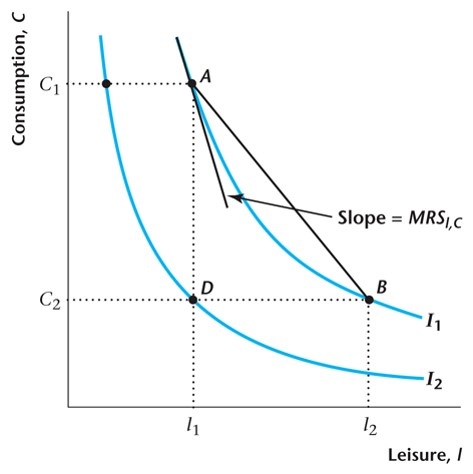
\includegraphics[width=\textwidth]{./figures/Figure4_2.jpg}
        \end{figure}
        \end{column}
    \end{columns}
\end{frame}

\section{Optimization}
\label{sec:Optimization}

\begin{frame}{Consumer's Problem}
\label{slide:Consumer_s_Problem}
    The consumer choose \alert{consumption} and \alert{leisure} bundle to achieve \alert{highest} indifference curve, while still satisfying \alert{budget constraint}
     %
     \begin{equation}
     \label{eq:HHProblem}
         \begin{split}
             \max_{C, l} \quad
                 & U( C, l )
             \\
             \text{subject to } \quad
                & C \le w( h - l ) + \pi - T
            \\
         \end{split}
     \end{equation}
     %
     \begin{itemize}
         \item \textbf{Rational behavior}: decision is made given preference \& constraints
         \item \textbf{Analysis}: both \alert{graphically} and \alert{algebraically}
     \end{itemize}
\end{frame}

\begin{frame}{Graphical Analysis: Interior Solution}
\label{slide:Graphical_Analysis__Interior_Solution}
    \begin{columns}
        \begin{column}{0.5\textwidth}
            \begin{itemize}
                \item \textbf{Interior}: sol. at middle of budget set, not end pts
                \item \alert{MRS} must equal to \alert{real wage} ($MRS_{l, C} = w$), WHY?
                \begin{itemize}
                    \item sacrificed consumption comes from the decrease of labor income
                \end{itemize}
                \item Sol. at indifference curve \alert{tangent} to budget set
                \item \textbf{Convexity}: E v.s. H \& F v.s. H
            \end{itemize}
        \end{column}
        \begin{column}{0.5\textwidth}
            \begin{figure}
                \caption{Figure 4.5 Interior Solution}
                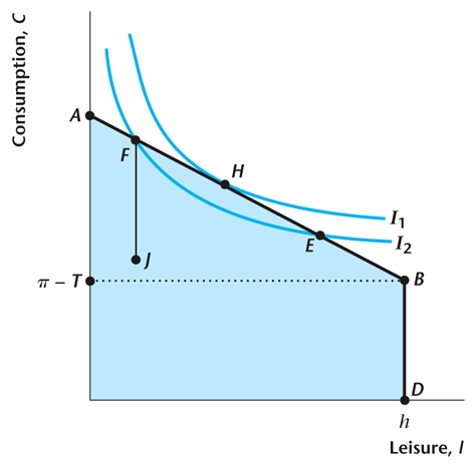
\includegraphics[width=\textwidth]{./figures/Figure4_5.jpg}
            \end{figure}
        \end{column}
    \end{columns}
\end{frame}

\begin{frame}{Graphical Analysis: Corner Solution}
\label{slide:Graphical_Analysis__Corner_Solution}
    \begin{columns}
        \begin{column}{0.5\textwidth}
            \begin{itemize}
                \item \textbf{Corner}: sol. at end pts of budget set
                \item \alert{MRS} \alert{NOT} equal to \alert{real wage} ($MRS_{l, C} \neq w$), WHY?
                \begin{itemize}
                    \item working limited to total $ h $ hours, ``kink''
                \end{itemize}
                \item Sol. is NOT tangent to indifference curve
                % \item \textbf{Convexity}: E v.s. H \& F v.s. H
            \end{itemize}
        \end{column}
        \begin{column}{0.5\textwidth}
            \begin{figure}
                \caption{Figure 4.6 Corner Solution}
                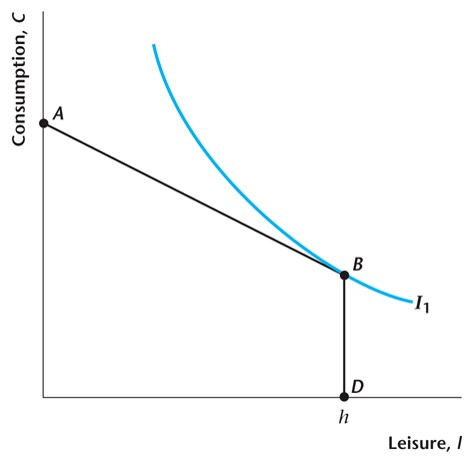
\includegraphics[width=\textwidth]{./figures/Figure4_6.jpg}
            \end{figure}
        \end{column}
    \end{columns}

\end{frame}

\begin{frame}{Algebraic Analysis: Interior Solution}
\label{slide:Algebraic_Analysis__Interior_Solution}
    Recall consumer's problem:
    %
    \begin{equation}
    \label{eq:HHProblem_recall}
        \begin{split}
            \max_{C, l} \quad
                & U( C, l )
            \\
            \text{subject to } \quad
               & C \le w( h - l ) + \pi - T
           \\
        \end{split}
    \end{equation}
    %
    \begin{itemize}
        \item Calculus is about \alert{derivative}: not defined at ``kink'' $ \Rightarrow  $ only \alert{interior sol.}
        \item Sol. at the \alert{border} of budget set $ \Rightarrow  $ budget constraint is ``$ = $'' (\alert{binding})
    \end{itemize}
    Plug the budget constraint into utility function to replace $ C $, we get
    %
    \begin{equation}
    \label{eq:HHProblem_plugin}
        \max_{l} \quad U( w( h-l ) + \pi - T, l )
    \end{equation}
    %
\end{frame}

\begin{frame}{Algebraic Analysis: Interior Solution (Cont.)}
\label{slide:Algebraic_Analysis__Interior_Solution__Cont__}
    %
    \begin{equation*}
        \max_{l} \quad U( w( h-l ) + \pi - T, l )
    \end{equation*}
    %
    Remember that now $ C = w( h-l ) + \pi - T $.
    Take \alert{first order condition} w.r.t. $ l $,
    %
    \begin{align}
        \overbrace{D_{C} U( C, l ) \times \frac{d [ w ( h-l ) + \pi - T ]}{d l}}^{\text{Derivative on $ C $ direction, \jump{slide:Chain_rule}{chain rule}}}
            & + \overbrace{D_{l} U( C, l )}^{\text{Derivative on $ l $ direction}} = 0
        \\
        D_{C}U( C, l ) \times ( -w )
            & + D_{l} U( C, l ) = 0
        \\
        w = \frac{D_{l}U( C, l )}{D_{C}U( C, l )}
            & = MRS_{l, C}
    \end{align}
    %
    Note: $ D_{x} f( \cdot ) $ is a shorthand for $ \frac{d f( \cdot )}{d x} $, meaning \alert{differentiation} of $ f( \cdot ) $ with respect to choice variable $ x $.
\end{frame}

\section{Experiment}
\label{sec:Experiment}

\begin{frame}{Build model for experiment}
\label{slide:Build_model_for_experiment}
    \begin{itemize}
        % \item Macroeconomists usually \textbf{cannot} do experiment: severe impact
        \item We want to know \alert{what's the result of changes}!
        \item Recall \alert{Lucas critique}: need to understand individual behavior
        \item Consider two experiments:
        \begin{enumerate}
            \item direct increase in \alert{real income} (no $ C $ and $ l $ trade off, pure \alert{income effect})
            \item increase in \alert{real wage} (\alert{income + substitution effect})
        \end{enumerate}
    \end{itemize}
\end{frame}

\begin{frame}{Experiment 1: Increase in dividends / Decrease in Tax}
\label{slide:Experiment_1__Increase_in_dividends}
    \begin{columns}
        \begin{column}{0.5\textwidth}
            \begin{itemize}
                \item \textbf{Recall}: $ C $ \& $ l $ are normal goods
                \item \textbf{Income effect}: income $ \uparrow  $ $ \Rightarrow  $ normal goods $ \uparrow  $
                \item Increase in dividends or decrease in taxes are level shifts up in real income, regardless of actions
                \item Consumer increases consumption, reduces quantity of labor supplied (increase leisure).
            \end{itemize}
        \end{column}
        \begin{column}{0.5\textwidth}
            \begin{figure}
                \caption{Figure 4.6 $ \pi \uparrow $ / $ T \downarrow  $}
                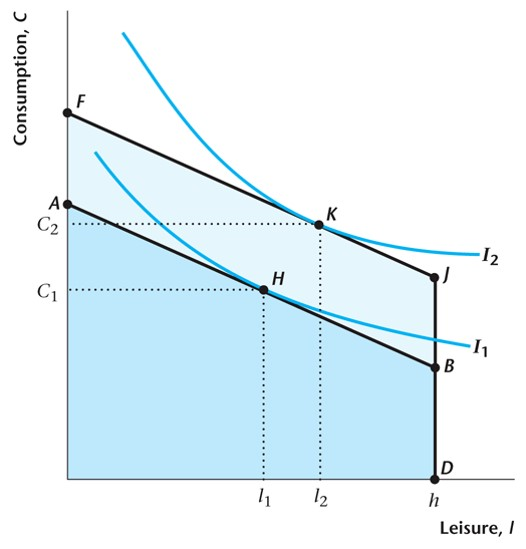
\includegraphics[width=\textwidth]{./figures/Figure4_7.jpg}
            \end{figure}
        \end{column}
    \end{columns}
\end{frame}

\begin{frame}{Experiment 2: Increase in Real Wage}
\label{slide:Experiment_2__Increase_in_Real_Wage}

    \begin{columns}
        \begin{column}{0.5\textwidth}
            \textbf{Substitution effect}: $ w \uparrow  $, leisure is costly, sacrifice $ l $ for $ C $
            \begin{itemize}
                \item budget line AB to JK, keeps F just affordable
                \item move along $ I_{1} $ : new slope of budget line
            \end{itemize}
            \textbf{Income effect}: income $ \uparrow  $ $ \Rightarrow  $ normal goods $ \uparrow  $
            \begin{itemize}
                \item budget line JK to EB, actual new budget line
                \item move up to $ I_{2} $: higher utility possible
            \end{itemize}
        \end{column}
        \begin{column}{0.5\textwidth}
            \begin{figure}
                \caption{Figure 4.8  $w \uparrow $, both effects canceled out}
                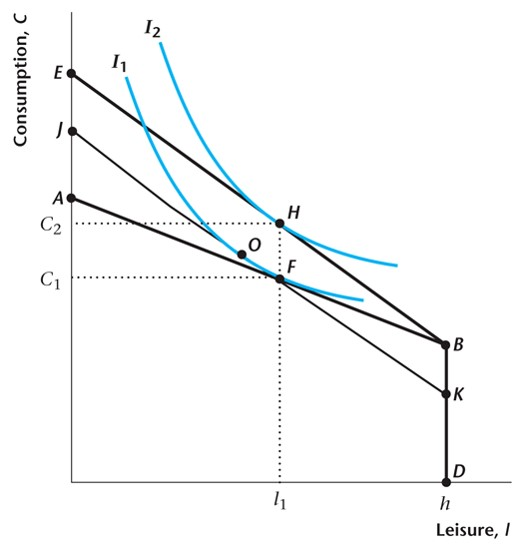
\includegraphics[width=\textwidth]{./figures/Figure4_8.jpg}
            \end{figure}
        \end{column}
    \end{columns}

\end{frame}

\begin{frame}{Experiment 1 \& 2: Labor Supply}
\label{slide:Experiment_1____2__Labor_Supply}

    \begin{columns}
        \begin{column}{0.5\textwidth}
        Looking ahead to putting the pieces together in a full model:
        \begin{itemize}
            \item Solution to consumer problem defines the supply curve for the labor market!
            \item What assumption ensures this is increasing in the wage?
            \begin{itemize}
                \item substitution effect: $ w \uparrow \Rightarrow l \downarrow (\text{i.e., } N^{S} \uparrow ) $
                \item income effect: $ w \uparrow \Rightarrow l \uparrow  (\text{i.e., } N^{S} \downarrow ) $
                \item Income effect $ < $ substitution effect
            \end{itemize}
        \end{itemize}
        \end{column}
        \begin{column}{0.5\textwidth}
            \begin{figure}
                \caption{Figure 4.10, LS on $ \pi \uparrow $ / $ T \downarrow  $}
                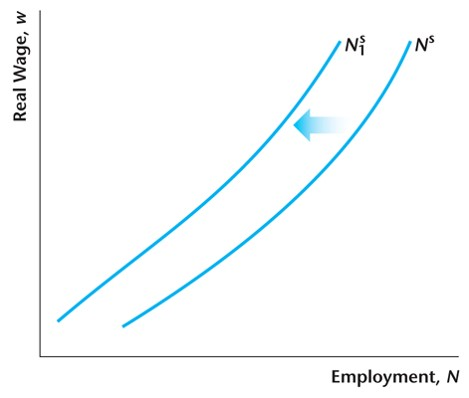
\includegraphics[width=\textwidth]{./figures/Figure4_10.jpg}
            \end{figure}
        \end{column}
    \end{columns}
\end{frame}

\section{Appendix}
\label{sec:Appendix}

\appendix
% -------------------------------------------
\setbeamertemplate{headline}
{
\setbeamercolor{section in head/foot}{fg=black, bg=white}
\vskip1em \tiny \insertsectionnavigationhorizontal{1\paperwidth}{\hspace{0.50\paperwidth}}{}
}
%------------------------------------------
\begin{frame}\frametitle{}
\begin{columns}
\label{Appendix}
\column{1\linewidth}
\centering
{\Large \alert{Appendix}}
\end{columns}
\end{frame}
%------------------------------------------

\begin{frame}{Chain rule}
\label{slide:Chain_rule}
\framesubtitle{\jump{slide:Algebraic_Analysis__Interior_Solution__Cont__}{Back}}
In the main slide, we applied \alert{chain rule} to the $ C $ direction of the $ U( C, l ) $. By binding budget constraints, we know $ C( l ) = w( h-l ) + \pi - T $, i.e., consumption is a function of leisure.

%
\begin{equation}
\label{eq:Chain rule}
    \frac{d}{dl} U( C( l ) ) = \frac{dU( C, l )}{dC} \times \frac{dC( l )}{dl} = D_{C} U( C, l ) \times D_{l} C( l )
\end{equation}
%
where $ D_{l}C( l ) = -w $.

\end{frame}

\end{document}
